\documentclass[conference]{IEEEtran}
\IEEEoverridecommandlockouts
% The preceding line is only needed to identify funding in the first footnote. If that is unneeded, please comment it out.
\usepackage{cite}
\usepackage{amsmath,amssymb,amsfonts}
\usepackage{algorithmic}
\usepackage{graphicx}
\usepackage{textcomp}
\usepackage{xcolor}
\usepackage[spanish]{babel}
\usepackage[utf8]{inputenc}
\usepackage{url}
\def\BibTeX{{\rm B\kern-.05em{\sc i\kern-.025em b}\kern-.08em
    T\kern-.1667em\lower.7ex\hbox{E}\kern-.125emX}}
\begin{document}

\title{Ciclo de Vida del Software: Modelo Espiral y Metodología Scrumban}

\author{\IEEEauthorblockN{Angel Luis Valdés Sánchez}
\IEEEauthorblockA{\textit{Maestría en Ingeniería de Software} \\
\textit{Universidad Tecnológica de la Mixteca}\\
Huajuapan de León, Oaxaca \\
angelluis2605@gs.utm.mx}
}

\pagestyle{plain}

\maketitle

\begin{abstract}
El ciclo de vida del desarrollo de software (SDLC, por sus siglas en inglés) constituye un marco fundamental para la gestión sistemática de proyectos de software. Este reporte examina los fundamentos generales del SDLC y realiza un análisis comparativo detallado entre dos enfoques metodológicos distintos: el Modelo Espiral, como representante de las metodologías tradicionales orientadas al manejo de riesgos, y Scrumban, como ejemplo de las metodologías ágiles híbridas. A través del análisis de casos de estudio reales, incluyendo el proyecto NASA TReK y implementaciones empresariales de Scrumban, se evalúan las fortalezas, limitaciones y contextos de aplicación óptimos para cada metodología. Los resultados indican que mientras el Modelo Espiral aventaja en proyectos complejos con altos riesgos y requisitos inciertos, Scrumban ofrece flexibilidad superior para equipos que requieren la estructura de Scrum combinada con la fluidez de Kanban.
\end{abstract}

\section{Introducción}

El desarrollo de software moderno enfrenta desafíos cada vez más complejos, caracterizados por requisitos cambiantes, plazos ajustados y la necesidad de entregar valor de manera continua \cite{dhiman2024reassessment}. En este contexto, la selección de un modelo de ciclo de vida del software adecuado se convierte en un factor crítico para el éxito del proyecto \cite{comparative_study_2020}.

El concepto de ciclo de vida del desarrollo de software ha evolucionado significativamente desde sus inicios en la década de 1970. Mientras que los enfoques tradicionales como el modelo en cascada proporcionaban estructura y predictibilidad, las metodologías modernas han incorporado principios de adaptabilidad y gestión de riesgos \cite{shylesh2017study}. Según estudios recientes, más del 50\% del software desarrollado nunca se utiliza, y más del 70\% no satisface los requisitos del usuario, lo que subraya la importancia de seleccionar el modelo SDLC apropiado \cite{ieee_comparative_2021}.

Este reporte se enfoca en dos metodologías representativas: el Modelo Espiral, propuesto por Barry Boehm en 1986 como una respuesta orientada al manejo de riesgos \cite{boehm1988spiral}, y Scrumban, una metodología híbrida que combina elementos de Scrum y Kanban para proporcionar flexibilidad en entornos ágiles \cite{zayat2020framework}. El objetivo es proporcionar un análisis comparativo basado en evidencia que ayude a los profesionales a tomar decisiones informadas sobre la selección metodológica.

\section{Fundamentos del Ciclo de Vida del Desarrollo de Software}

\subsection{Definición y Propósito del SDLC}

El ciclo de vida del desarrollo de software se define como un proceso estructurado que describe las fases involucradas en el desarrollo de sistemas de información \cite{contemporary_sdlc_2023}. Este marco proporciona una metodología sistemática para planificar, crear, probar y desplegar sistemas de software de alta calidad \cite{dhiman2024reassessment}.

Los componentes fundamentales del SDLC incluyen: análisis de requisitos, diseño del sistema, implementación, pruebas, despliegue y mantenimiento \cite{wang2025survey}. Cada fase tiene objetivos específicos, entregables definidos y criterios de finalización claros \cite{contemporary_sdlc_2023}. 

Según Sommerville \cite{sommerville2016}, estas fases constituyen un marco genérico aplicable a la mayoría de los procesos de software:

\begin{itemize}
    \item \textbf{Especificación de requisitos:} se identifican y documentan las necesidades del cliente y las restricciones del sistema.
    \item \textbf{Diseño y desarrollo:} se transforman los requisitos en una representación arquitectónica y detallada que guiará la construcción del software.
    \item \textbf{Implementación y validación:} se construye el sistema y se realizan pruebas para asegurar que cumple con los requisitos definidos.
    \item \textbf{Evolución o mantenimiento:} se realizan modificaciones para corregir errores, mejorar el rendimiento o adaptarse a cambios en el entorno y en los requisitos.
\end{itemize}

Este modelo genérico proporciona una base común sobre la cual se han desarrollado variantes más específicas como el modelo en cascada, el modelo espiral y metodologías ágiles.

\subsection{Evolución de los Modelos SDLC}

La evolución de los modelos SDLC refleja la maduración de la ingeniería de software como disciplina. Los modelos tradicionales, caracterizados por enfoques secuenciales y orientados a la documentación, han dado paso a metodologías más flexibles y adaptativas \cite{comprehensive_review_2023}.

Estudios contemporáneos indican que aproximadamente el 60\% de los \textit{benchmarks} o criterios actuales se enfocan en la fase de desarrollo dentro del SDLC, mientras que la ingeniería de requisitos y el diseño de software reciben atención mínima con solo 5\% y 3\% respectivamente \cite{wang2025survey}. Esta disparidad destaca la necesidad de modelos que equilibren todas las fases del desarrollo.

\subsection{Criterios de Selección de Modelos}

La selección de un modelo SDLC apropiado depende de múltiples factores, incluyendo la complejidad del proyecto, el nivel de incertidumbre, el tamaño del equipo y las restricciones organizacionales \cite{comparative_study_2020}. La investigación indica que diferentes enfoques son más efectivos según las características específicas del proyecto y el contexto organizacional \cite{ganjeizadeh2015statistical}.

% TODO: Falta hablar mas sobre el ciclo de vida y cada una de las fases para cada metodología.

\section{Modelo Espiral: Un Enfoque Tradicional Orientado al Riesgo}

\subsection{Fundamentos Teóricos}

El Modelo Espiral, introducido por Barry W. Boehm en 1986 \cite{boehm1988spiral}, representa un enfoque evolutivo orientado al manejo de riesgos que combina elementos del modelo en cascada con desarrollo iterativo \cite{boehm1988spiral}. El modelo se caracteriza por su representación gráfica en espiral, donde el radio representa el costo acumulativo del proyecto y el progreso angular indica el avance a través del proceso de desarrollo \cite{techtarget_spiral}.

Boehm diseñó el modelo como un meta-modelo que puede acomodar cualquier proceso de desarrollo apropiado, utilizando la evaluación de riesgos como mecanismo de selección \cite{semantic_scholar_spiral}. Esta característica distintiva permite al modelo adaptarse a diferentes contextos de proyecto manteniendo un enfoque sistemático en la identificación y mitigación de riesgos \cite{boehm1988spiral}.

\subsection{Estructura y Fases del Modelo}

El Modelo Espiral opera a través de cuatro cuadrantes principales \cite{ultimate_sdlc_spiral}:

\begin{enumerate}
\item \textbf{Determinación de objetivos, alternativas y restricciones}: Los requisitos del sistema se definen con el mayor detalle posible, incluyendo artefactos para funcionalidad, rendimiento e interfaces \cite{ultimate_sdlc_spiral}.

\item \textbf{Identificación y resolución de riesgos}: Se evalúan todas las alternativas disponibles para desarrollar un proyecto costo-efectivo, identificando riesgos como falta de experiencia, tecnología nueva o cronogramas ajustados \cite{gordon_case_study}.

\item \textbf{Desarrollo y pruebas}: Se crea un prototipo del sistema basado en el diseño preliminar, siguiendo el patrón habitual de crear y revisar el diseño, codificar, inspeccionar código y probar el producto \cite{ultimate_sdlc_spiral}.

\item \textbf{Planificación}: Se desarrollan planes de proyecto, gestión de configuración, pruebas e instalación \cite{gordon_case_study}.
\end{enumerate}

\subsection{Fases del Ciclo de Vida en el Modelo Espiral}

El Modelo Espiral organiza el desarrollo en ciclos sucesivos, donde cada iteración recorre actividades similares a las fases clásicas del SDLC, pero con un énfasis central en la identificación y mitigación de riesgos. La Figura~\ref{fig:espiral} ilustra gráficamente estas fases y su relación con el progreso del proyecto.

\begin{itemize}
    \item \textbf{Determinación de objetivos y requisitos:} en cada vuelta de la espiral se definen metas específicas, considerando funcionalidades a implementar, restricciones técnicas y alternativas viables.
    \item \textbf{Análisis de riesgos y planificación:} se identifican posibles amenazas técnicas, de costos o cronogramas, y se proponen estrategias de mitigación. Esta fase distingue al modelo espiral de otros enfoques secuenciales.
    \item \textbf{Desarrollo y validación:} se crean prototipos o incrementos de software, combinando diseño, implementación y pruebas para validar tempranamente con los interesados.
    \item \textbf{Revisión y preparación de la siguiente iteración:} al finalizar cada ciclo, se validan resultados, se ajusta la planificación y se define el alcance de la próxima vuelta de la espiral.
\end{itemize}

\begin{figure}[h]
    \centering
    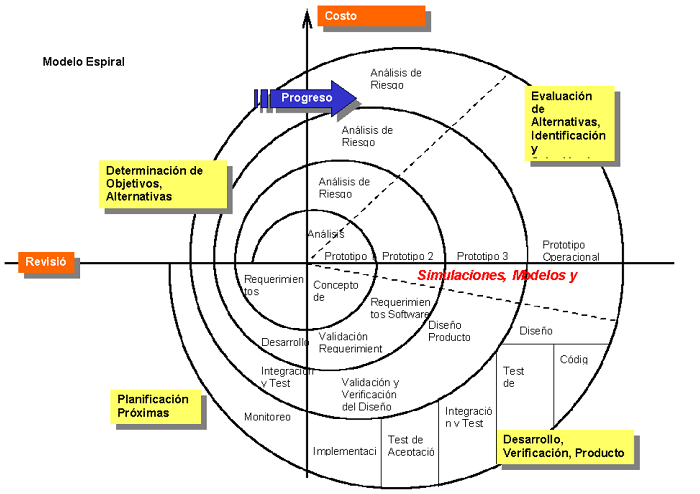
\includegraphics[width=0.48\textwidth]{espiral.png}
    \caption{Representación gráfica del Modelo Espiral, mostrando sus fases iterativas orientadas al manejo de riesgos (Figura 2 del artículo de Olivera, 2021 \cite{olivera2021redalyc}).}
    \label{fig:espiral}
\end{figure}

Este enfoque asegura que cada fase del ciclo de vida no se aborda de manera rígida y secuencial, sino como parte de un proceso iterativo en el que se reduce la incertidumbre progresivamente \cite{boehm1988spiral}.

\subsection{Casos de Estudio: NASA TReK y TRW-SPS}

\subsubsection{NASA TReK Project}

El proyecto TReK de la NASA representa una aplicación exitosa del Modelo Espiral en un entorno de alta complejidad técnica \cite{nasa_trek_2002}. El proyecto enfrentó numerosos desafíos incluyendo restricciones presupuestarias, limitaciones temporales y el fenómeno de ``\textit{requirements creep}'' o desviación incontrolable del alcance \cite{nasa_trek_2002}.

La implementación del Modelo Espiral permitió al equipo identificar y mitigar riesgos críticos de manera temprana, resultando en una entrega exitosa a pesar de las restricciones significativas. El enfoque iterativo facilitó la adaptación a cambios en los requisitos regulatorios y técnicos durante el desarrollo \cite{nasa_trek_2002}.

\subsubsection{TRW Software Productivity System}

Boehm utilizó el Modelo Espiral para desarrollar el Sistema TRW-SPS, un proyecto complejo que resultó en 1,300,000 instrucciones de computadora \cite{sciencedirect_spiral}. Se aplicó un estudio de factibilidad llamado ``\textit{Round Zero}'' para determinar si el proyecto TRW-SPS representaba valor significativo para la organización \cite{sciencedirect_spiral}.

El estudio de factibilidad indicó que el proyecto era viable (bajo riesgo), permitiendo que el proyecto se expandiera hacia afuera en la espiral. Los entregables de rondas posteriores incluyeron múltiples pasos repetidos, incluyendo desarrollo de prototipos y, más importante, análisis de riesgos \cite{sciencedirect_spiral}.

\subsection{Ventajas y Limitaciones}

\textbf{Ventajas del Modelo Espiral:}
\begin{itemize}
\item Manejo sistemático de riesgos a través de análisis continuo \cite{geeksforgeeks_spiral}
\item Flexibilidad para adaptarse a proyectos con requisitos inciertos \cite{boehm1988spiral}
\item Capacidad para incorporar elementos de otros modelos según sea necesario \cite{semantic_scholar_spiral}
\item Enfoque iterativo que permite refinamiento continuo \cite{teaching_agile_spiral}
\end{itemize}

\textbf{Limitaciones:}
\begin{itemize}
\item Complejidad de gestión que puede ser excesiva para proyectos pequeños \cite{geeksforgeeks_spiral}
\item Tiempo considerable requerido para evaluación de riesgos y prototipado \cite{gordon_case_study}
\item Necesidad de experiencia especializada en análisis de riesgos \cite{nelson_small_project}
\item Potencial para espirales indefinidas sin criterios de finalización claros \cite{ultimate_sdlc_spiral}
\end{itemize}

\section{Scrumban: Una Metodología Ágil Híbrida}

\subsection{Fundamentos Conceptuales}

Scrumban emerge como una metodología híbrida que combina la estructura organizacional de Scrum con la flexibilidad de flujo de trabajo de Kanban \cite{atlassian_scrumban}. Esta aproximación híbrida fue inicialmente desarrollada como un mecanismo de transición para equipos que migraban entre metodologías, pero ha evolucionado hacia un sistema maduro capaz de manejar proyectos complejos y continuos \cite{atlassian_scrumban}.

La metodología se fundamenta en principios clave que incluyen la visualización del flujo de trabajo, limitación del trabajo en progreso (WIP, por sus siglas en inglés), flujo continuo de trabajo y mejora iterativa \cite{sixsigma_scrumban}. Estos principios permiten a los equipos mantener la predictibilidad de Scrum mientras aprovechan la adaptabilidad inherente de Kanban \cite{empirical_scrumban_2018}.

\subsection{Características Distintivas}

Scrumban incorpora elementos específicos de ambas metodologías padre \cite{comparison_agile_2016}:

\textbf{De Scrum:}
\begin{itemize}
\item Reuniones diarias de seguimiento
\item Retrospectivas para análisis de desempeño
\item Roles definidos incluyendo el \textit{Scrum Master}
\item \textit{Sprints} con duraciones flexibles (típicamente no superiores a dos semanas) \cite{comparison_agile_2016}
\end{itemize}

\textbf{De Kanban:}
\begin{itemize}
\item Tableros visuales para gestión de flujo de trabajo
\item Límites de trabajo en progreso
\item Flujo continuo sin restricciones temporales estrictas
\item Métricas de flujo y tiempo de ciclo \cite{kanban_vs_scrum}
\end{itemize}

\subsection{Fases del Ciclo de Vida en Scrumban}

En contraste con los modelos secuenciales, Scrumban gestiona el ciclo de vida de manera continua y dinámica. Sus fases no son estrictamente lineales, sino que coexisten dentro del flujo de trabajo visualizado en los tableros Kanban. La Figura~\ref{fig:scrumban} ilustra este ciclo, donde la planificación, ejecución, revisión y mejora continua se integran de manera iterativa.

\begin{itemize}
    \item \textbf{Planificación ligera:} se definen objetivos inmediatos y se priorizan las tareas a través de un \textit{backlog} flexible.
    \item \textbf{Ejecución iterativa:} las tareas se mueven a través del tablero visual, limitando el trabajo en progreso (WIP) para mantener un flujo sostenible.
    \item \textbf{Revisión y retroalimentación:} al finalizar cada conjunto de tareas o mini-\textit{sprint}, el equipo evalúa el progreso y ajusta prioridades.
    \item \textbf{Mejora continua:} las retrospectivas y métricas de flujo permiten refinar procesos, reducir desperdicios y mejorar la calidad del producto.
\end{itemize}

\begin{figure}[h]
    \centering
    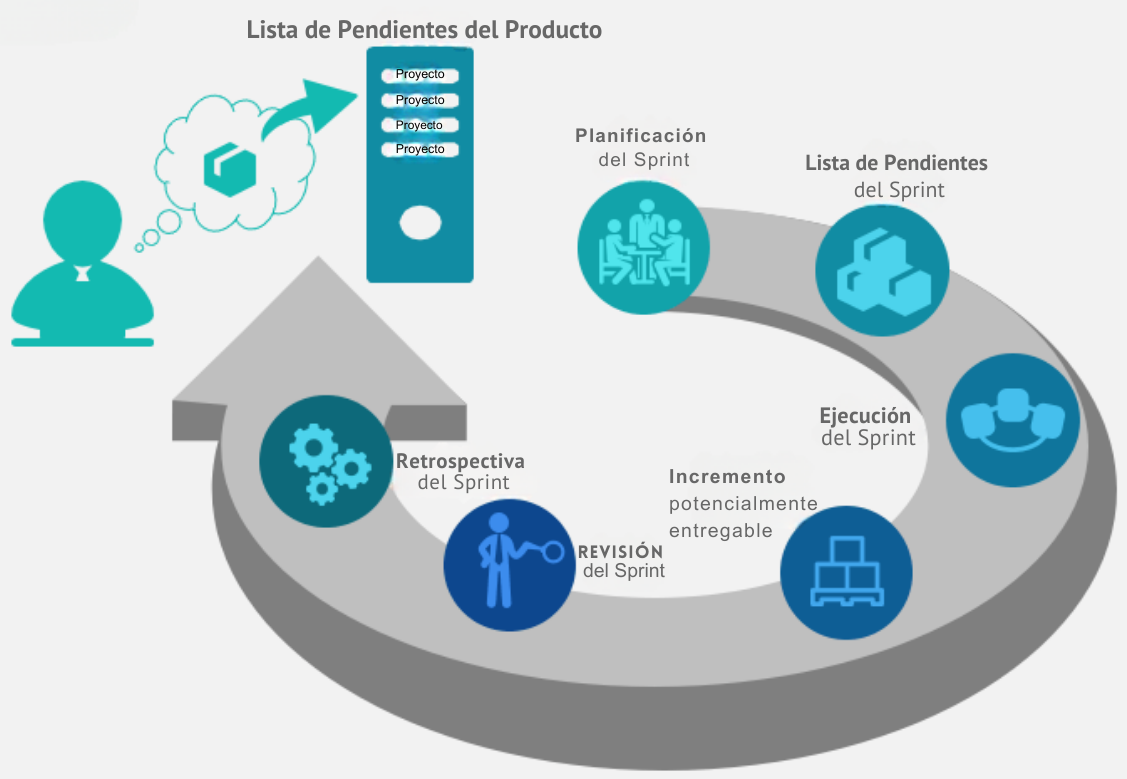
\includegraphics[width=0.48\textwidth]{scrumban.png}
    \caption{Representación de las fases iterativas en Scrumban (elaboración propia adaptada de recursos en línea).}
    \label{fig:scrumban}
\end{figure}

Estas fases no tienen límites temporales rígidos; más bien, se integran en un ciclo continuo que favorece la adaptabilidad y la entrega constante de valor \cite{atlassian_scrumban, sixsigma_scrumban}.

\subsection{Casos de Estudio de Implementación}

\subsubsection{Transición Scrum a Scrumban en Empresa Tecnológica}

Un estudio de caso documentó es la transición de Scrum a Scrumban en una empresa de desarrollo de software vietnamita \cite{scrum_to_scrumban_2012}. La investigación utilizó un enfoque de investigación-acción para analizar el proceso de transición, los cambios implementados en el proceso de desarrollo y las mejoras logradas \cite{scrum_to_scrumban_2012}.

Los resultados mostraron mejoras significativas en la gestión del flujo de trabajo, reducción en el tiempo de entrega y mayor satisfacción del equipo. La flexibilidad adicional proporcionada por Scrumban permitió al equipo adaptarse mejor a cambios en los requisitos sin comprometer la entrega continua \cite{scrum_to_scrumban_2012}.

\subsubsection{Implementación con Gamificación en Turquía}

Un caso de estudio empírico realizado en una empresa mediana en Turquía demostró la implementación exitosa de Scrumban combinado con elementos de gamificación \cite{yilmaz_gamification_2016}. El estudio involucró a 30 profesionales trabajando en el mismo proyecto dentro de un centro de investigación tecnológica \cite{yilmaz_gamification_2016}.

Los resultados preliminares indicaron que la integración de elementos de juego con la metodología híbrida Scrumban mejoró la productividad individual y organizacional. El análisis estadístico mostró una diferencia de 0.5 puntos en la escala Likert entre las mediciones pre y post implementación, con un valor t calculado (6.12) superior al valor crítico de tabla (1.79) \cite{yilmaz_gamification_2016}.

\subsubsection{Estudios de Formación de Scrumban}

La investigación sobre la formación de prácticas Scrumban revela que los equipos ágiles familiarizados con tanto Scrum como Kanban pueden combinar y beneficiarse más de Scrumban \cite{empirical_scrumban_formation}. El estudio identifica factores que asisten a los miembros del equipo ágil en la formación exitosa de Scrumban mediante la combinación apropiada de prácticas de Kanban y Scrum \cite{empirical_scrumban_2018}.

Los hallazgos indican que Scrumban resulta más apropiado que Scrum o Kanban individualmente para ahorrar tiempo, mejorar calidad y minimizar desperdicios \cite{empirical_scrumban_2018}.

\subsection{Ventajas y Desafíos}

\textbf{Ventajas de Scrumban:}
\begin{itemize}
\item Flexibilidad superior para adaptarse a cambios de requisitos \cite{sixsigma_scrumban}
\item Combinación efectiva de estructura y fluidez \cite{atlassian_scrumban}
\item Reducción del tiempo de ciclo de desarrollo \cite{agile_marketing_examples}
\item Mejora en la transparencia y comunicación del equipo \cite{yilmaz_gamification_2016}
\item Capacidad para manejar trabajos de mantenimiento y desarrollo simultáneamente \cite{scrumbanfall_2020}
\end{itemize}

\textbf{Desafíos:}
\begin{itemize}
\item Requiere experiencia previa en ambas metodologías (Scrum y Kanban) \cite{empirical_scrumban_2018}
\item Complejidad inicial en la configuración del proceso híbrido \cite{scrumban_integration_2020}
\item Necesidad de adaptación cultural organizacional \cite{yilmaz_gamification_2016}
\item Riesgo de inconsistencia en la aplicación sin guías claras \cite{scrumbanfall_2020}
\end{itemize}

\section{Análisis Comparativo y Casos de Estudio}

\subsection{Análisis Comparativo Metodológico}

La comparación entre el Modelo Espiral y Scrumban revela diferencias fundamentales en filosofía, aplicación y contextos óptimos de uso. Mientras el Modelo Espiral prioriza la mitigación sistemática de riesgos a través de análisis exhaustivo y prototipado iterativo \cite{boehm1988spiral}, Scrumban enfatiza la adaptabilidad continua y la entrega de valor incremental \cite{atlassian_scrumban}.

\textbf{Gestión de Riesgos:}
El Modelo Espiral incorpora análisis de riesgos como actividad central en cada iteración \cite{boehm1988spiral}, mientras que Scrumban maneja riesgos a través de entregas frecuentes y feedback continuo del cliente \cite{sixsigma_scrumban}. Estudios empíricos muestran que el Modelo Espiral es superior para proyectos con riesgos técnicos altos y requisitos inciertos \cite{teaching_agile_spiral}, mientras que Scrumban excele en entornos con cambios frecuentes de prioridades \cite{ganjeizadeh2015statistical}.

\textbf{Flexibilidad vs. Estructura:}
El análisis estadístico de implementaciones muestra que Kanban (componente de Scrumban) supera ligeramente a Scrum en el factor de cronograma \cite{ganjeizadeh2015statistical}. Sin embargo, el Modelo Espiral proporciona mayor predictibilidad en proyectos de largo plazo debido a su enfoque de planificación exhaustiva \cite{nasa_trek_2002}.

\subsection{Contextos de Aplicación Óptimos}

\textbf{Modelo Espiral - Contextos Apropiados:}
\begin{itemize}
\item Proyectos de alta complejidad técnica (sistemas espaciales, software crítico) \cite{nasa_trek_2002}
\item Duraciones de 6 meses a 2 años \cite{ultimate_sdlc_spiral}
\item Presupuestos significativos (mayor a \$3M) \cite{ultimate_sdlc_spiral}
\item Equipos con experiencia en análisis de riesgos \cite{nelson_small_project}
\item Requisitos con alta incertidumbre inicial \cite{boehm1988spiral}
\end{itemize}

\textbf{Scrumban - Contextos Apropiados:}
\begin{itemize}
\item Equipos de desarrollo ágil con experiencia previa \cite{empirical_scrumban_2018}
\item Proyectos con requisitos cambiantes frecuentemente \cite{sixsigma_scrumban}
\item Entornos que requieren entrega continua \cite{atlassian_scrumban}
\item Organizaciones que buscan balance entre estructura y flexibilidad \cite{yilmaz_gamification_2016}
\item Proyectos de mantenimiento y desarrollo simultáneo \cite{scrumbanfall_2020}
\end{itemize}


\section{Conclusión}

Este análisis comparativo del Modelo Espiral y Scrumban revela que ambas metodologías ofrecen ventajas distintivas según el contexto del proyecto. El Modelo Espiral demuestra superioridad en proyectos de alta complejidad y riesgo, como evidenciado por su aplicación exitosa en proyectos como NASA TReK y TRW-SPS. Su enfoque sistemático en la gestión de riesgos y la capacidad para adaptarse a requisitos inciertos lo convierten en la opción preferida para proyectos críticos de gran escala.

Por el contrario, Scrumban ofrece la flexibilidad necesaria para entornos de desarrollo modernos caracterizados por cambios frecuentes de requisitos y la necesidad de entrega continua. Los casos de estudio analizados demuestran mejoras significativas en satisfacción del equipo, tiempo de ciclo y adaptabilidad organizacional.

La selección entre estas metodologías debe basarse en una evaluación cuidadosa de factores como complejidad del proyecto, tolerancia al riesgo, experiencia del equipo y características organizacionales. Futuras investigaciones deberían enfocarse en desarrollar marcos de decisión cuantitativos que faciliten la selección metodológica basada en características específicas del proyecto.

Los hallazgos de este estudio contribuyen al cuerpo de conocimiento en ingeniería de software al proporcionar evidencia empírica sobre la aplicabilidad contextual de diferentes modelos SDLC, facilitando decisiones informadas para profesionales y organizaciones en la selección de metodologías de desarrollo de software.

\begin{thebibliography}{00}
\bibitem{dhiman2024reassessment} K. L. Dhiman, ``Reassessment of Software Development Life Cycle Models,'' \emph{International Journal of Research in Engineering, Science and Management}, vol. 7, no. 2, pp. 4--10, Feb. 2024.

\bibitem{comparative_study_2020} ``Software Development Life Cycle Models-A Comparative Study,'' \emph{ResearchGate}, July 2020. [Online]. Available: \url{https://www.researchgate.net/publication/346819120_Software_Development_Life_Cycle_Models-A_Comparative_Study}

\bibitem{shylesh2017study} S. S. Shylesh, ``A Study of Software Development Life Cycle Process Models,'' \emph{SSRN}, June 2017. [Online]. Available: \url{https://papers.ssrn.com/sol3/papers.cfm?abstract_id=2988291}

\bibitem{wang2025survey} K. Wang et al., ``Software Development Life Cycle Perspective: A Survey of Benchmarks for Code Large Language Models and Agents,'' \emph{arXiv preprint arXiv:2505.05283}, May 2025.

\bibitem{ieee_comparative_2021} ``Comparative Analysis of Software Life Cycle Models,'' \emph{IEEE Conference Publication}, IEEE Xplore. [Online]. Available: \url{https://ieeexplore.ieee.org/document/9362931/}

\bibitem{contemporary_sdlc_2023} ``Research on Contemporary Software Development Life Cycle Models,'' \emph{American Journal of Computer Science and Technology}, Science Publishing Group, Mar. 2023.

\bibitem{comprehensive_review_2023} ``A Comprehensive Review of Software Development Life Cycle methodologies: Pros, Cons, and Future Directions,'' \emph{Iraqi Journal for Computer Science and Mathematics}, July 2023.

\bibitem{boehm1988spiral} B. W. Boehm, ``A spiral model of software development and enhancement,'' \emph{Computer}, vol. 21, no. 5, pp. 61--72, May 1988.

\bibitem{zayat2020framework} W. Zayat and O. Senvar, ``Framework Study for Agile Software Development Via Scrum and Kanban,'' \emph{ResearchGate}, July 2020.

\bibitem{techtarget_spiral} ``What is the Spiral Model and How is It Used?,'' \emph{TechTarget}. [Online]. Available: \url{https://www.techtarget.com/searchsoftwarequality/definition/spiral-model}

\bibitem{semantic_scholar_spiral} B. W. Boehm, ``A spiral model of software development and enhancement,'' \emph{Semantic Scholar}, 1986.

\bibitem{ultimate_sdlc_spiral} ``The Spiral Model - The Ultimate Guide to the SDLC,'' \emph{Ultimate SDLC}, 2023.

\bibitem{gordon_case_study} D. T. Gordon, ``Spiral Model in Software Engineering with Case Study,'' \emph{SlideShare}.

\bibitem{nasa_trek_2002} ``NASA's TReK project: a case study in using the spiral model of software development,'' \emph{Communications of the ACM}, vol. 45, no. 4, 2002.

\bibitem{sciencedirect_spiral} ``Spiral Model - an overview,'' \emph{ScienceDirect Topics}.

\bibitem{geeksforgeeks_spiral} ``What is Spiral Model in Software Engineering?,'' \emph{GeeksforGeeks}, Mar. 2018.

\bibitem{teaching_agile_spiral} ``Spiral Model in Software Development: Guide to Risk-Driven Development,'' \emph{Teaching Agile}, Apr. 2023.

\bibitem{nelson_small_project} H. C. Nelson, ``Applying the spiral model: A case study in small project management,'' \emph{Wiley Online Library}, Dec. 1998.

\bibitem{atlassian_scrumban} ``Scrumban: Mastering Two Agile Methodologies,'' \emph{Atlassian}, Apr. 2025.

\bibitem{sixsigma_scrumban} ``Scrumban: Hybrid Methodology of Scrum and Kanban,'' \emph{SixSigma.us}, July 2024.

\bibitem{empirical_scrumban_2018} ``An Empirical Study of Scrumban Formation based on the Selection of Scrum and Kanban Practices,'' \emph{ResearchGate}, Dec. 2018.

\bibitem{comparison_agile_2016} ``Comparison of agile methods: Scrum, Kanban, and Scrumban,'' \emph{ResearchGate}, Oct. 2016.

\bibitem{kanban_vs_scrum} ``Kanban vs. scrum: which agile are you?,'' \emph{Atlassian}, Apr. 2025.

\bibitem{scrum_to_scrumban_2012} ``From Scrum to Scrumban: a case study of a process transition,'' \emph{ResearchGate}, June 2012.

\bibitem{yilmaz_gamification_2016} M. Yilmaz and R. V. O'Connor, ``A Scrumban Integrated Gamification Approach To Guide Software Process Improvement: A Turkish Case Study,'' \emph{ResearchGate}, Feb. 2016.

\bibitem{empirical_scrumban_formation} ``An Empirical Study of Scrumban Formation based on the Selection of Scrum and Kanban Practices,'' \emph{ResearchGate}, Dec. 2018.

\bibitem{scrumbanfall_2020} ``Scrumbanfall: An Agile Integration of Scrum and Kanban with Waterfall in Software Engineering,'' \emph{ResearchGate}, Feb. 2020.

\bibitem{scrumban_integration_2020} ``Scrumban: An Agile Integration of Scrum and Kanban in Software Engineering,'' \emph{ResearchGate}, Feb. 2020.

\bibitem{ganjeizadeh2015statistical} F. Ganjeizadeh et al., ``A statistical analysis of the effects of Scrum and Kanban on software development projects,'' \emph{ScienceDirect}, Dec. 2015.

\bibitem{agile_marketing_examples} ``Agile Marketing Examples \& Case Studies,'' \emph{AgileSherpas}.

\bibitem{sommerville2016} I. Sommerville, \emph{Ingeniería de Software}, 10ª ed., Pearson, 2016.

\bibitem{olivera2021redalyc}
L.\,C. Olivera, “Modelos de Desarrollo de Software,” \emph{Revista de Investigación 3783}, Redalyc, 2021, figura 2. Disponible: \url{https://www.redalyc.org/journal/3783/378366538003/html/}

\end{thebibliography}
\vspace{12pt}

\end{document}
